\documentclass[../root]{subfiles}
\graphicspath{{_images/}{../_images/}}


\begin{document}

    \chapter{The Hidden Costs of Control}

    \begin{shortsummary}
        \begin{itemize}
            \item \authoryear{Falk2006}
            \item \RQ{How does the agent perceive the principal's decision to control?
                      How does control affect the agent's behavior?}
            \item \answer{An experimental principal-agent game 
                          (Principal can control the agent by implementing a minimum performance request)}
            \item \result{A principal's control reduces an agent's performance, but a principal's payoff is non-monotonic.}
        \end{itemize}
    \end{shortsummary}

    \section{Introduction}

    \begin{itemize}
        \item Critical problem of principal-agent relations is \textbf{a conflict of interest}.
        \begin{itemize}
            \item effort $x \in \mathbb{R}_+$ is costly to the agent, and the principal's payoff is increasing in effort $x$.
            \item In standard economics, the agent will choose $x = 0$, which leads to the lowest payoff of the principal.
        \end{itemize}
        \item Two common ways to eliminate agents' actions against a principal's interest.
        \begin{enumerate}
            \item Restrict agent's choice set: $x \in [\underline{x}, +\infty)$
            \item Incentivize agents to take actions following a principal's interest: the agent's payoff is $\pi_A(x) = bx - C(x)$ where $b > 0$.
        \end{enumerate}
        \item This paper proposes that \textbf{agents who are intrinsically motivated to perform the principal's interest may decrease performance by control because they perceive control as a negative signal of distrust (control aversion)}.
        \item To test their hypothesis, they implement a laboratory experiment, which is that the principal can force the agent to choose at least a minimum effort level before the agent chooses effort level.
        \begin{itemize}
            \item Finding 1: A majority of the agents choose a lower effort $x$ if the principal restricts rather than trusts them.
            \item Finding 2: The net effect on profits is non-monotonic, that is, control generates significantly lower profits than trust for low levels of $\underline{x}$, while control breaks even for high levels of $\underline{x}$. 
        \end{itemize} 
        \item This result provides the psychological rationale for the \textit{deliberate} incomplete contract.
        \begin{itemize}
            \item Real-life contracts often omit important, verifiable obligations of the contracting parties.
            \item When the principal expects the hidden cost of control, the principal implements a less complete contract.
        \end{itemize}
    \end{itemize}
    
    \section{Experimental Design}

    \begin{table}[h]
        \centering
        \caption{Between Treatment Design}
        \begin{tabular}{c|ccc}
            \hline
            Treatment & 
            Principal's choice & 
            Agent's choice &
            \# Subjects\\
            \hline
            C5  &
            $\underline{x} \in \{0,5\}$ & 
            \dlinecell{$x \in \{\underline{x}, \ldots, 120\}$ in each $\underline{x}$ \\ before learning $\underline{x}$} &
            140 \\
            C10 & 
            $\underline{x} \in \{0,10\}$ & 
            \dlinecell{$x \in \{\underline{x}, \ldots, 120\}$ in each $\underline{x}$ \\ before learning $\underline{x}$} &
            144 \\
            C20 &
            $\underline{x} \in \{0,20\}$ &
            \dlinecell{$x \in \{\underline{x}, \ldots, 120\}$ in each $\underline{x}$ \\ before learning $\underline{x}$} &
            134 \\
            SR10 & 
            $\underline{x} \in \{0,10\}$ & 
            $x \in \{\underline{x}, \ldots, 120\}$ after learning &
            246 \\
            EX10 &
            no decision &
            $x \in \{10, \ldots, 120\}$ &
            72 \\
            GE10 &
            \dlinecell{$\underline{x} \in \{0,10\}$ and \\ $w \in \{10, 30, 60, 120\}$} &
            \dlinecell{$x \in \{\underline{x}, \ldots, 120\}$ in each $(\underline{x}, w)$ \\ 
                       before learning $(\underline{x}, w)$} &
            68 \\
            \hline
        \end{tabular}
    \end{table}

    \begin{itemize}
        \item Payoff functions
        \begin{itemize}
            \item C5, C10, C20, SR10 and EX10: $\pi_p = 2x$ and $\pi_a = 120 - x$
            \item GE10: $\pi_p = 2x - w$ and $\pi_a = w - x$.
        \end{itemize}
        \item Other features of the design
        \begin{itemize}
            \item Timing of decision: (i) principal's choice, (ii) agent's choice
            \item Each principal-agent game was played one-shot.
            \item Subjects were randomly allocated a role as principal or as agent upon arrival at the lab.
        \end{itemize}
        \item Predictions
        \begin{itemize}
            \item C5, C10, and C20: we can investigate whether the effect of controlling on the principal's payoff is non-monotonic.
            \item C10 vs EX10: Control aversion predicts that $x$-choices should be higher in the EX10 than in the C10 (Outcome-based preference predicts no difference).
            \item C10 vs SR10: Authors use the strategy method in the main treatments (ask $x$ in each principal's action before knowing the principal's actual decision). By this method, the agents may understate (overstate) their dislike for control.
            \item C10 vs GE10: Wages are introduced to approximate real-world employment relations. In the standard social-preference, effort $x$ increases as wage $w$ increases. For higher wages, control may not be optimal since the principal can signal his trust by not choosing control.  
        \end{itemize}
    \end{itemize}

    \section{Results}

    \subsection{Agent's Decision-Making}

    \begin{figure}[h]
        \centering
        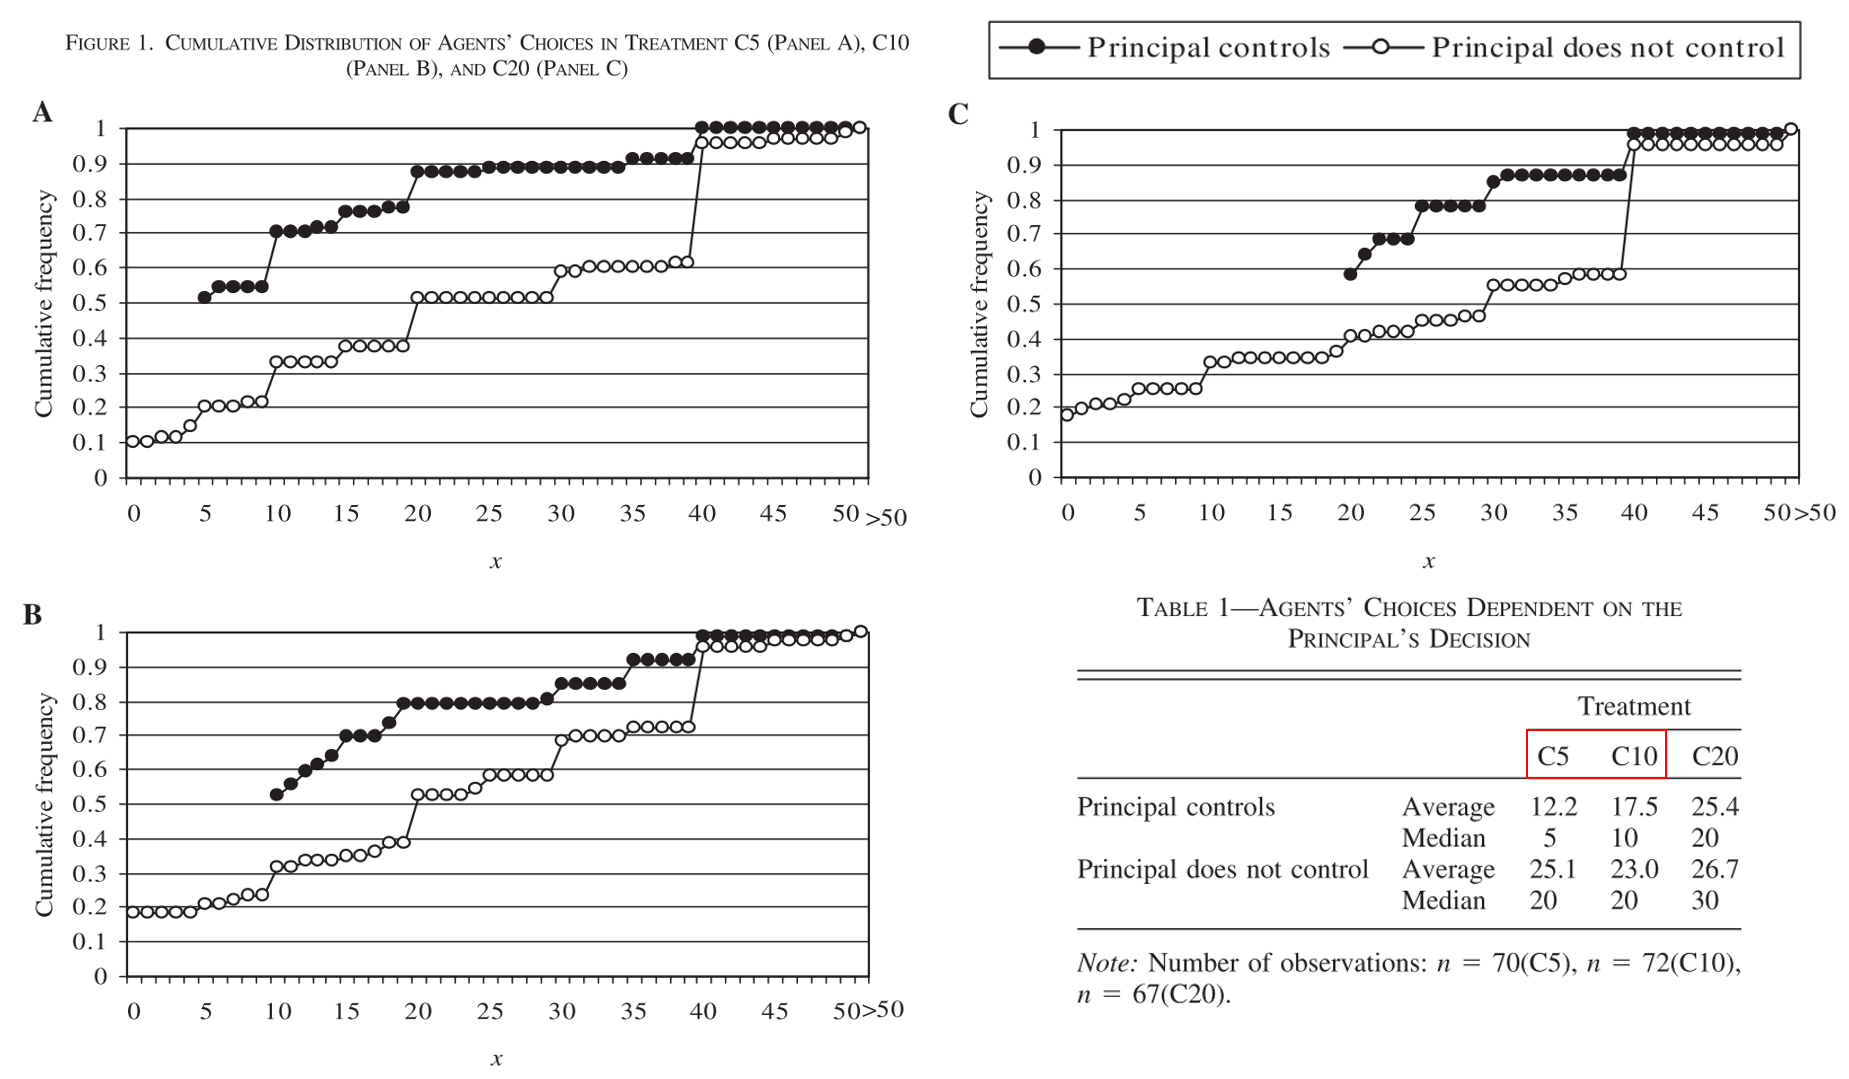
\includegraphics[width = 16cm]{0515kato/result1.pdf}
        \caption{Main Result of Agent's Decision-Making}
        \label{result1}
    \end{figure}

    \begin{figure}[h]
        \centering
        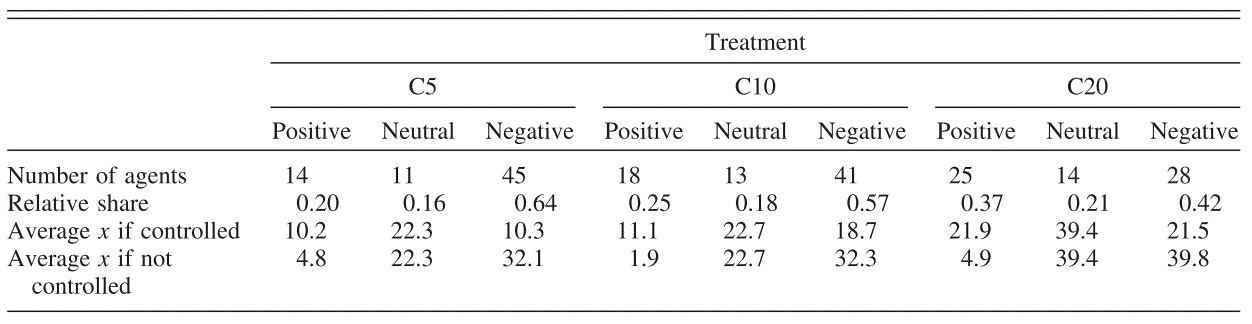
\includegraphics[width = 16cm]{0515kato/result2.png}
        \caption{Heterogeneity of Agent's Decision-Making}
        \label{result2}
    \end{figure}

    \begin{itemize}
        \item Result 1: We observe the hidden costs of control in all main treatments. Average performance is higher if the principal does not control than if he does so. These differences are significant in the C5 and the C10, but not in the C20 (See Figure \ref{result1}).
        \begin{itemize}
            \item Agents do not behave differently if the principal does not control. This suggests that agents seem to punish the principal's decision to control rather than reward his decision to trust.
        \end{itemize}
        \item Result 2: There is a strong heterogeneity among the agents in all main treatments. We see agents who react positively, neutrally, or negatively to the principal's implementation of control. The last group is always the majority (See Figure \ref{result2}).
        \begin{itemize}
            \item This result shows that the costs of control are substantial. However, this does not suggest that trust is always better than control.
            \item The difference in average profits between controlling and trusting is -25.8 in C5, -11.0 in C10, and -2.6 in C20.
            \item This implies that \textit{if the principal has only weak incentives at his disposal, it may be better to trust, since controlling lowers motivation of the intrinsically motivated agents but increases the performance of opportunistic agents only marginally}.
        \end{itemize}
        \item Robustness 1: There is no any effect of using the strategy method versus the specific response method (See Table \ref{robust1}).
        \begin{table}[h]
            \centering
            \caption{Robustness of Agent's Behavior}
            \label{robust1}
            \begin{tabular}{lccc}
                \hline
                &
                C10 &
                SR10 &
                Mann-Whitney test\\
                \hline 
                Principals control &
                17.5 &
                19.6 &
                0.589 \\
                &
                (10) &
                (10.5) \\
                Principals do not control &
                23.0 &
                23.6 &
                0.822 \\
                &
                (20) &
                (20) \\
                \hline
            \end{tabular}
        \end{table}
        \item Robustness 2: $x$-choices in the EX10 treatment exceed those in the C10 subgame following the control decision (See Table \ref{robust2}).
        \begin{table}[h]
            \centering
            \caption{Result of EX10 Treatment}
            \label{robust2}
            \begin{tabular}{lccccc}
                \hline
                &
                EX10 &
                \dlinecell{C10 \\ (control)} &
                \dlinecell{C10 \\ (trust)} &
                \dlinecell{MW test \\ (EX10 vs. C10 control)}  &
                \dlinecell{MW test \\ (EX10 vs. C10 trust)}  \\
                \hline 
                Average &
                28.7 &
                17.5 &
                23.0 &
                $<0.001$ &
                0.523 \\
                Median &
                20 &
                10 &
                20 &
                & \\
                \hline
            \end{tabular}
        \end{table}
        \item Robustness 3: Agents who are controlled think that the principal has lower expectations than do agents who are not controlled in the SR10 treatment.
        \begin{itemize}
            \item After the agent had made his decision, he answered the question, "What do you think were the expectations of participant B (principal) concerning your transfer decision?"
            \item In addition to signals of distrust, agents who believe that the principal has lowe expectations may feel less guilty when choosing a low $x$.
            \item Agents' transfers ($x$) and beliefs are significantly and positively correlated.
        \end{itemize}
        \item Robustness 4: most agents who reacted negatively to control in the experiment felt distrust and lack of autonomy.
    \end{itemize}

    \subsection{Principal's Decision-Making}

    \begin{figure}[h]
        \centering
        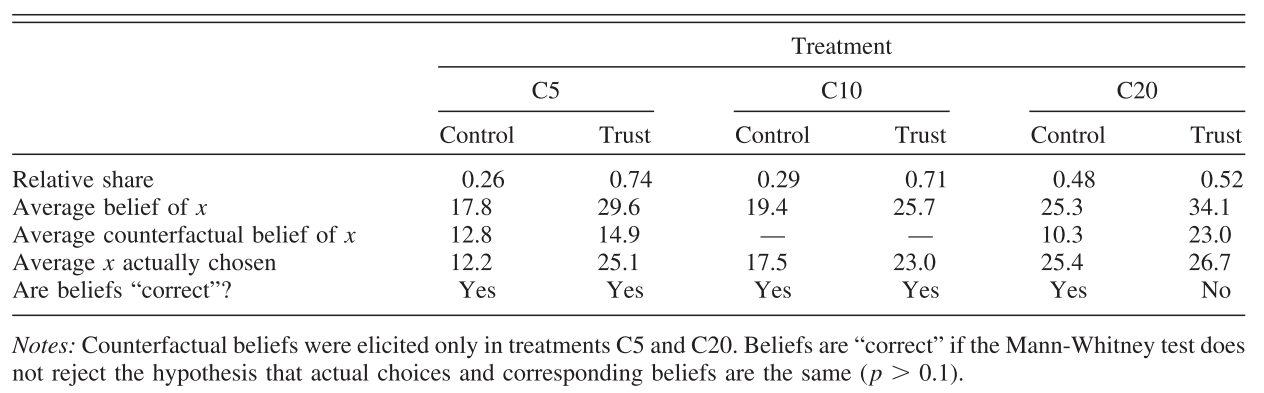
\includegraphics[width = 16cm]{0515kato/result3.png}
        \caption{Behavior and Beliefs of Principals}
        \label{result3}
    \end{figure}

    \begin{itemize}
        \item Result 3: The majority of the principals choose not to control the agent. Principals who control have lower expectations about $x$ than principals who do not. Expectations coincide with agents' average performance in most of the cases.
        \begin{itemize}
            \item In both the C5 and C20 treatments, principals who think that they get more if they control than if they trust choose to control, and vice versa. In this sense, principals' behavior is rational (コメント:beliefは選択のあとに聞いているので、自身の行動を合理化するような回答をしているかもしれない).
            \item Self-fulfilling prophecy of distrust: \textit{Principals who have rather pessimistic beliefs and hence choose to restrict the agent's choice set experience that their beliefs are indeed confirmed by their agents' relatively low average performance}.
        \end{itemize}
    \end{itemize}

    \subsection{Gift-Exchange Game}

    \begin{figure}[h]
        \centering
        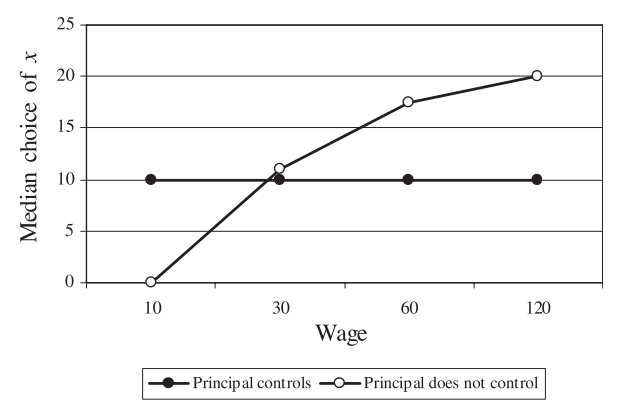
\includegraphics[width = 16cm]{0515kato/result4.png}
        \caption{Results of GE10 Treatment}
        \label{result4}
    \end{figure}

    \begin{itemize}
        \item Result 4: We observe reciprocity in the gift-exchange treatment, i.e., a positive relationship between wages and effort. Reciprocity is significantly weaker, however, if the principal controls than if he does not control (see Figure \ref{result4}).
        \begin{itemize}
            \item Linear regression of performance on wages: $\beta = 0.1909$ in the control condition, and $\beta = 0.2538$ in the no control condition, which are statistically significant.
            \item The net benefits of control are decreasing in wages, i.e., the negative effect of control on reciprocal agents is slightly stronger than the positive effect of control on selfish agents.
        \end{itemize}
    \end{itemize}

    \section{Concluding Remarks}

    \begin{quote}
        The main message of our paper is that control and explicit incentives entail hidden costs,
        which should be taken seriously.
        The message is \textit{not}, however, that it is always better for principals to trust than to control.
        In fact, we show that the costs and benefits of controlling agents depend on various factors.
        First, they depend on the composition of agents' type.
        \dots
        Second, the strength of the explicit incentives is important (\citealp[p.1628]{Falk2006}).
    \end{quote}

    \biblio

\end{document}